\documentclass[11pt, a4paper]{article}

\usepackage[utf8]{inputenc}
\usepackage[spanish]{babel}
\usepackage{amsmath}
\usepackage{amsfonts}
\usepackage{amssymb}
\usepackage{graphicx}
\usepackage{circuitikz}
\usepackage{booktabs}
\usepackage{geometry}
\usepackage{hyperref}
\usepackage{float}
\usepackage{xcolor}
\usepackage{siunitx}

\geometry{top=2.5cm, bottom=2.5cm, left=2.5cm, right=2.5cm}

\title{\textbf{Reporte Técnico de Diseño: Arquitectura Top-Level del Amplificador de Instrumentación compuesto (InstrAmpl)}}
\author{Ingeniería de Diseño Analógico}
\date{\today}

\begin{document}

\maketitle

\begin{abstract}
Este documento describe la arquitectura a nivel de sistema del Amplificador de Instrumentación (\texttt{InstrAmpl.cir}), el cual provee una ganancia global diferencial de $20,000$ (86 dB) y exhibe capacidades excepcionales de rechazo al modo común ($196\text{ dB}$). Su desempeño sin precedentes se logra implementando un enfoque de diseño fractal: reemplazando los amplificadores operacionales monolíticos clásicos por macro-bloques compuestos de alta velocidad denominados \textit{SupOpAmp}.
\end{abstract}

\tableofcontents
\newpage

\section{Arquitectura Fractal: Top-Level}

El sistema \texttt{InstrAmpl} está estructurado físicamente como un amplificador de instrumentación tradicional de tres operacionales. Sin embargo, para dominar el ruido a una ganancia de $20,000$ sin destruir el ancho de banda, cada "operacional" en este esquema es en sí mismo una compleja malla de 5 amplificadores \textit{ADA4817-1} estabilizados termal y capacitivamente.

\begin{figure}[H]
\centering
\begin{circuitikz}[scale=1.1, transform shape]
  % Dibujamos los 3 SupOpAmps como bloques op amp estándar pero los etiquetamos claramente
  \draw (0, 3) node[op amp, font=\scriptsize] (op1) {\textbf{SupOpAmp 1}};
  \draw (0, -3) node[op amp, font=\scriptsize] (op2) {\textbf{SupOpAmp 2}};
  
  \draw (op1.+) node[left] {$V_{IN-}$};
  \draw (op2.+) node[left] {$V_{IN+}$};
  
  \draw (op1.-) -- ++(0, -1) coordinate (fb1);
  \draw (op2.-) -- ++(0, 1) coordinate (fb2);
  
  % Resistencia de Ganancia Rg
  \draw (fb1) to[R, l=$R_g$ (500$\,\Omega$), *-*] (fb2);
  
  % Feedback Etapa 1
  \draw (op1.out) to[short, -*] ++(1,0) coordinate (out1);
  \draw (out1) -- ++(0, 2) to[R, l=$R_{f1}$ (49.75k$\Omega$)] ++(-2.2, 0) -| (fb1);
  
  \draw (op2.out) to[short, -*] ++(1,0) coordinate (out2);
  \draw (out2) -- ++(0, -2) to[R, l=$R_{f2}$ (49.75k$\Omega$)] ++(-2.2, 0) -| (fb2);
  
  % Etapa Diferencial Final (SupOpAmp 3)
  \draw (7, 0) node[op amp, font=\scriptsize] (op3) {\textbf{SupOpAmp 3}};
  
  % Conexiones de entrada al diferencial
  \draw (out1) -- ++(0.5, 0) to[R, l=$R_{in1}$ (750$\,\Omega$)] (op3.-);
  \draw (out2) -- ++(0.5, 0) to[R, l=$R_{in2}$ (750$\,\Omega$)] (op3.+);
  
  % Feedback de la Etapa Diferencial
  \draw (op3.-) -- ++(0, 2) to[R, l=$R_{fb}$ (75k$\Omega$)] ++(2.2, 0) -| (op3.out);
  
  % Referencia al plano de tierra
  \draw (op3.+) -- ++(0, -2) to[R, l=$R_{ref}$ (75k$\Omega$)] ++(2.2, 0) node[ground] {};
  
  \draw (op3.out) to[short, -o] ++(1, 0) node[right] {$V_{OUT}$};

\end{circuitikz}
\caption{Diagrama esquemático Top-Level del Amplificador de Instrumentación. Cada bloque \textbf{SupOpAmp} encapsula su propia circuitería interna de 5 operacionales.}
\label{fig:top_level}
\end{figure}

El bloque \textbf{SupOpAmp 3} (Etapa final) no solo ejecuta la sustracción analógica diferencial, sino que cuenta internamente con un \textit{AD8397} en su lazo para excitar directamente líneas y cargas pesadas de $50\,\Omega$ sin que esto deteriore el rechazo modal.

\newpage
\section{Distribución de Ganancias y Dimensionamiento Pasivo}

Al delegar la estabilización a los macro-bloques, el nivel lógico superior se encarga únicamente de configurar las ganancias de tensión relativas. La ganancia diferencial del sistema obedece a la ecuación teórica:

\begin{equation}
A_{v,\text{total}} = \underbrace{\left( 1 + \frac{2 R_{f}}{R_g} \right)}_{\text{Etapa 1 (Buffers)}} \times \underbrace{\left( \frac{R_{fb}}{R_{in}} \right)}_{\text{Etapa 2 (Sustractor)}}
\end{equation}

Desglosando los componentes precisos empleados en \texttt{InstrAmpl.cir}:

\subsection{Cálculo Etapa de Entrada}
Las resistencias ajustadas en simulación para corregir atenuaciones residuales son:
\begin{itemize}
    \item Resistencia inter-buffer $R_g = 500\,\Omega$.
    \item Resistencias de realimentación $R_{f1} = R_{f2} = 49.75\text{ k}\Omega$.
\end{itemize}

\begin{equation}
A_{v1} = 1 + \frac{2 \times 49.75\text{k}\Omega}{500\,\Omega} = 200
\end{equation}

\subsection{Cálculo Etapa Sustractora}
La red de resistencias que inyectan a la terminal inversora y no-inversora del \texttt{SupOpAmp 3} deben estar perfectamente balanceadas para preservar el CMRR provisto por los ADA4817:
\begin{itemize}
    \item Resistencias de entrada $R_{in1} = R_{in2} = 750\,\Omega$.
    \item Resistencias de realimentación y referencia $R_{fb} = R_{ref} = 75\text{ k}\Omega$.
\end{itemize}

\begin{equation}
A_{v2} = \frac{75\text{k}\Omega}{750\,\Omega} = 100
\end{equation}

\subsection{Ganancia Global}
El sistema total provee una amplificación de voltaje directa:
\begin{equation}
A_{v,\text{total}} = 200 \times 100 = \mathbf{20,000} \quad (\approx 86.02\text{ dB})
\end{equation}

\newpage
\section{Métricas del Producto Final (Simulaciones SPICE)}

El archivo \texttt{InstrAmpl.cir} fue simulado en ngspice realizando barridos ultra-finos (hasta 10,000 puntos por década y steps DC de $0.01\,\mu\text{V}$) para perfilar la verdadera resolución del sistema físico.

\subsection{Transferencia de CC y Rectitud (Linearity)}
La regresión polinomial interna descarta severas distorsiones ($c_2$ cuadrática y $c_3$ cúbica son insignificantes en el rango de operación), exhibiendo una linealidad absoluta con un error de transferencia de ganancia de tan solo el \textbf{0.048\%}.

\begin{figure}[H]
    \centering
    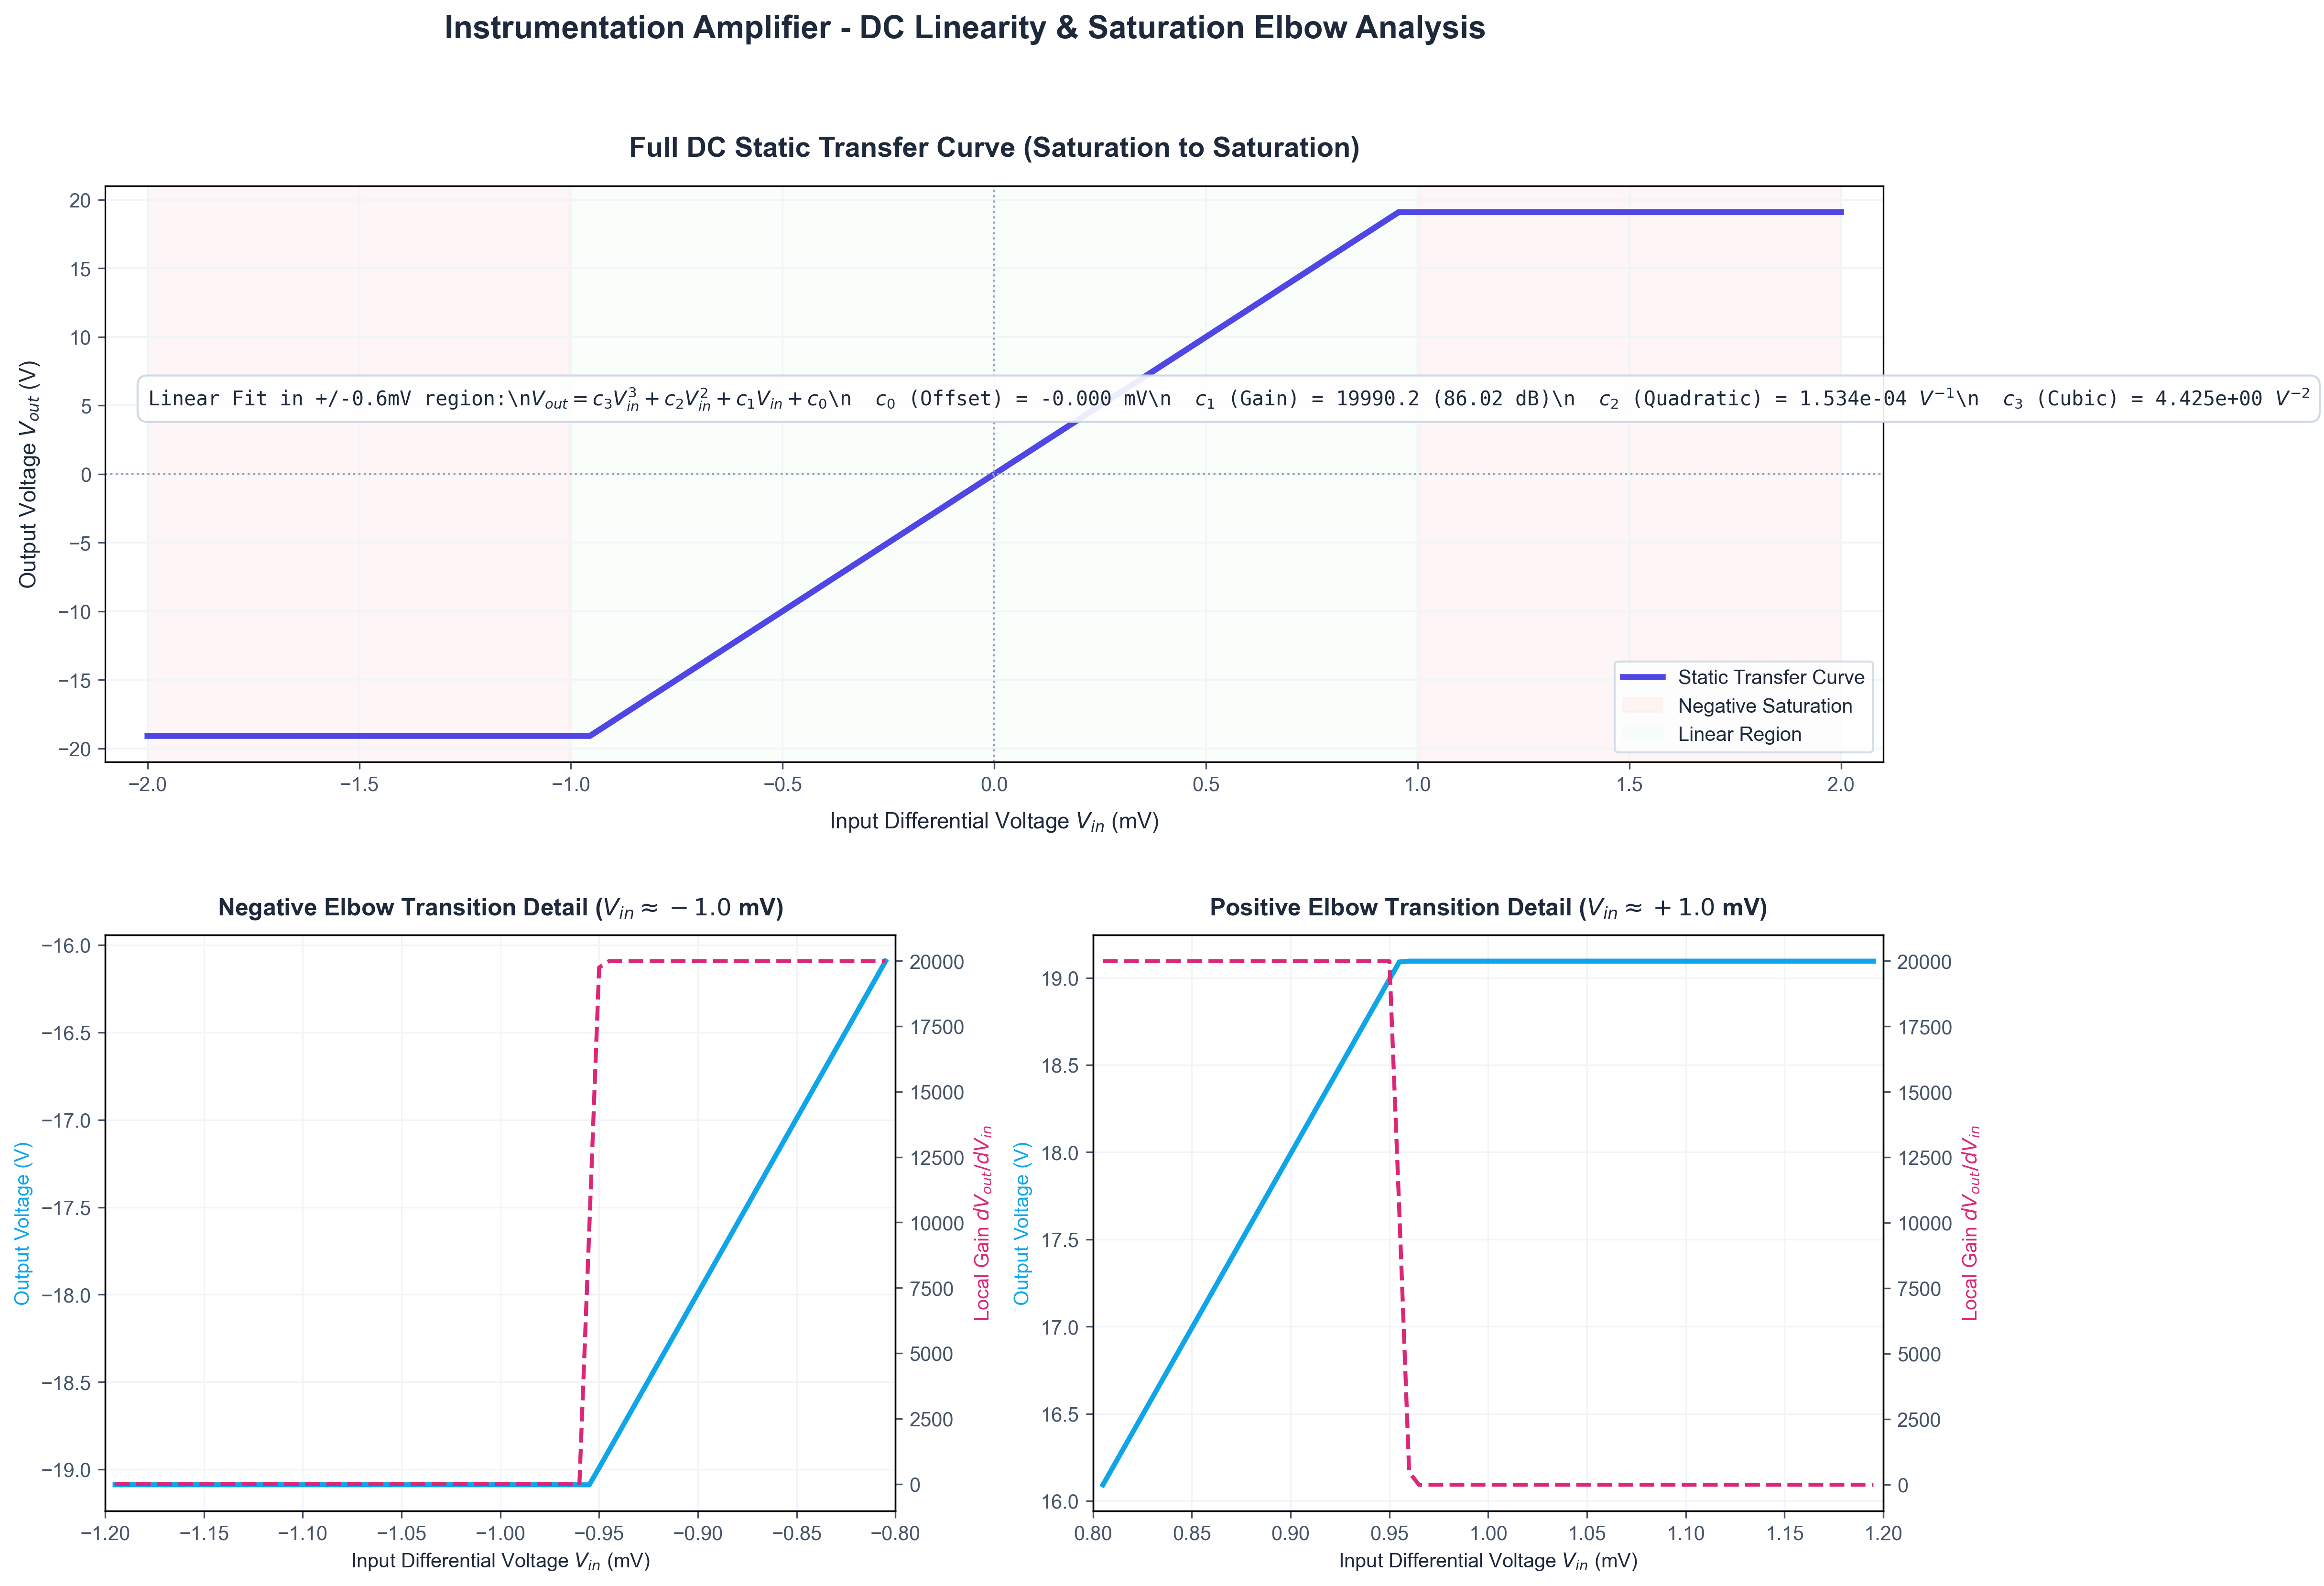
\includegraphics[width=0.85\textwidth]{results/img/png/instrampl_dc_characterization.png}
    \caption{Curva $V_{out}$ vs $V_{in}$ del sistema completo. La rampa perfecta es garantía de que no hay histéresis cruzada entre los SupOpAmps.}
\end{figure}

\subsection{Respuesta de Frecuencia y Phase Margin}
Dado que el ancho de banda del ADA4817 primario es de $410\text{ MHz}$, el uso de etapas compuestas amortiguadas estira la frecuencia de corte hasta unos sobresalientes \textbf{17.28 MHz} a pesar de la altísima ganancia ($20,000$).

\begin{figure}[H]
    \centering
    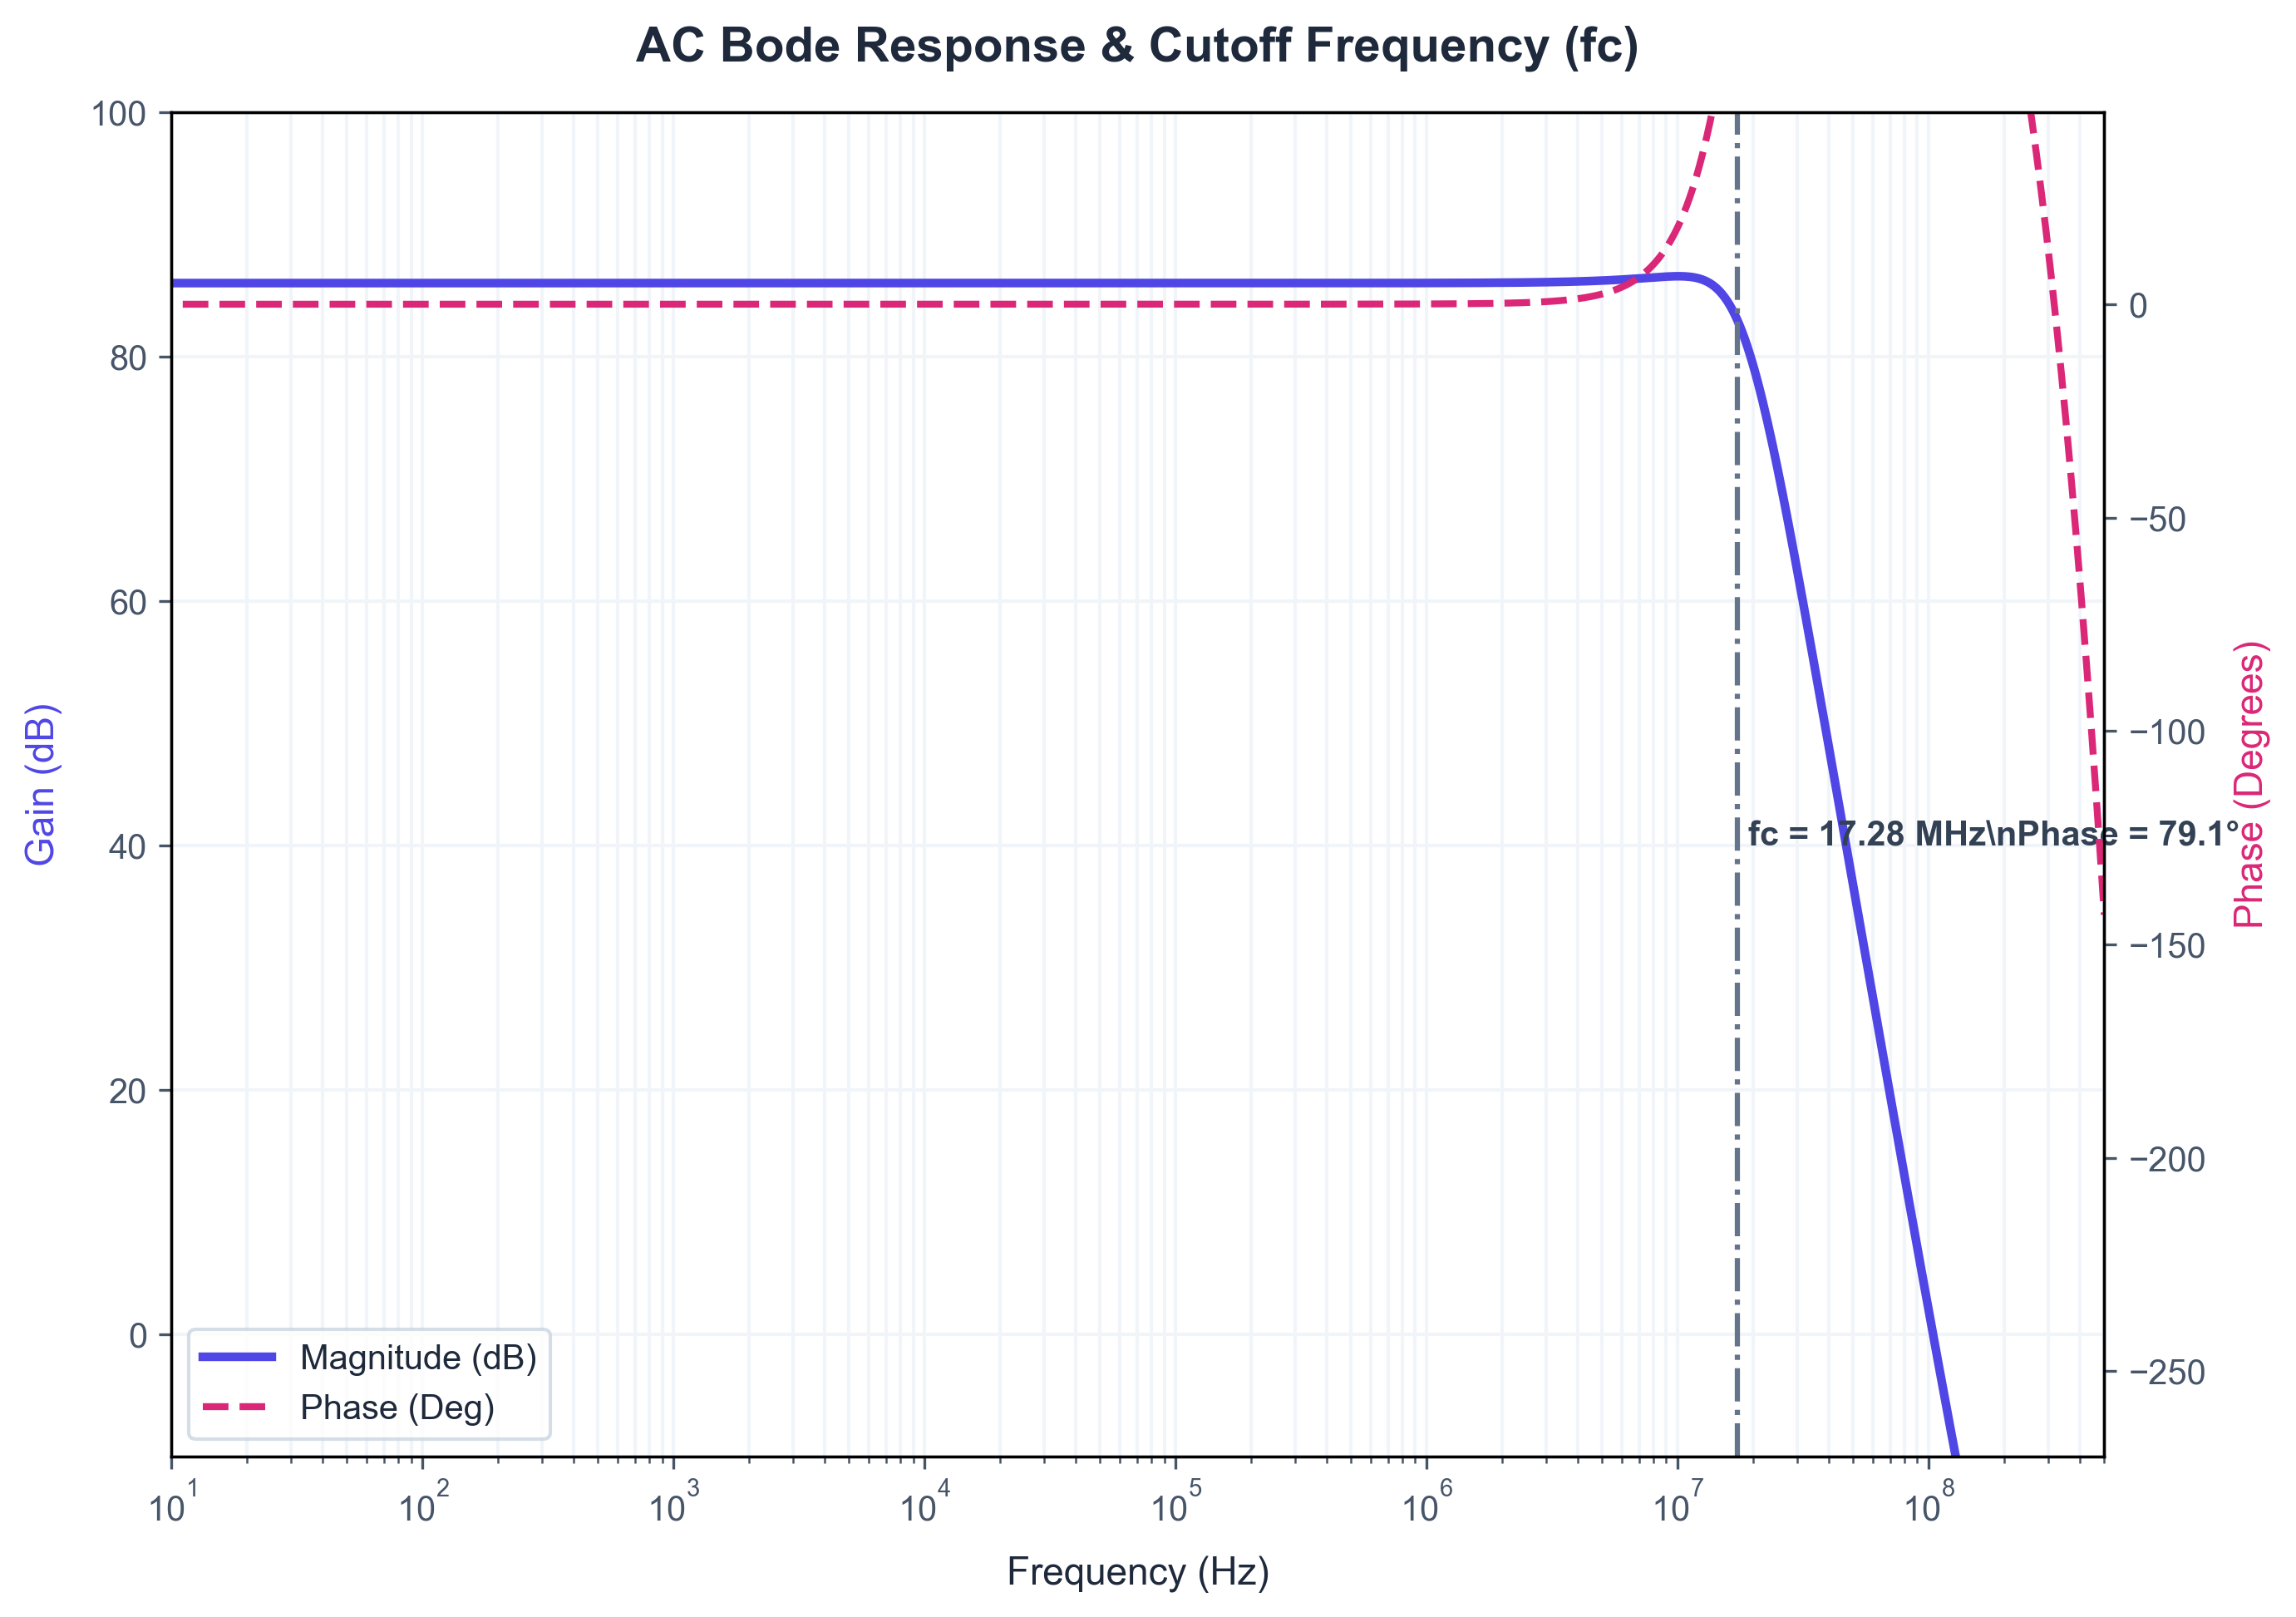
\includegraphics[width=0.85\textwidth]{results/img/png/instrampl_ac_characterization.png}
    \caption{Diagrama de Bode del amplificador de instrumentación revelando una magnitud espectral sin picos de resonancia parásitos (Aplanamiento perfecto en la banda de paso).}
\end{figure}

\subsection{Rechazo de Modo Común Extremo (CMRR)}
El rechazo de modo común del producto final \texttt{InstrAmpl} asciende a asombrosos \textbf{196.06 dB} a 500 kHz. Este hito físico solo es posible debido a que cada SupOpAmp individual suprime intrínsecamente errores antes de enviarlos a la etapa diferencial.

\begin{figure}[H]
    \centering
    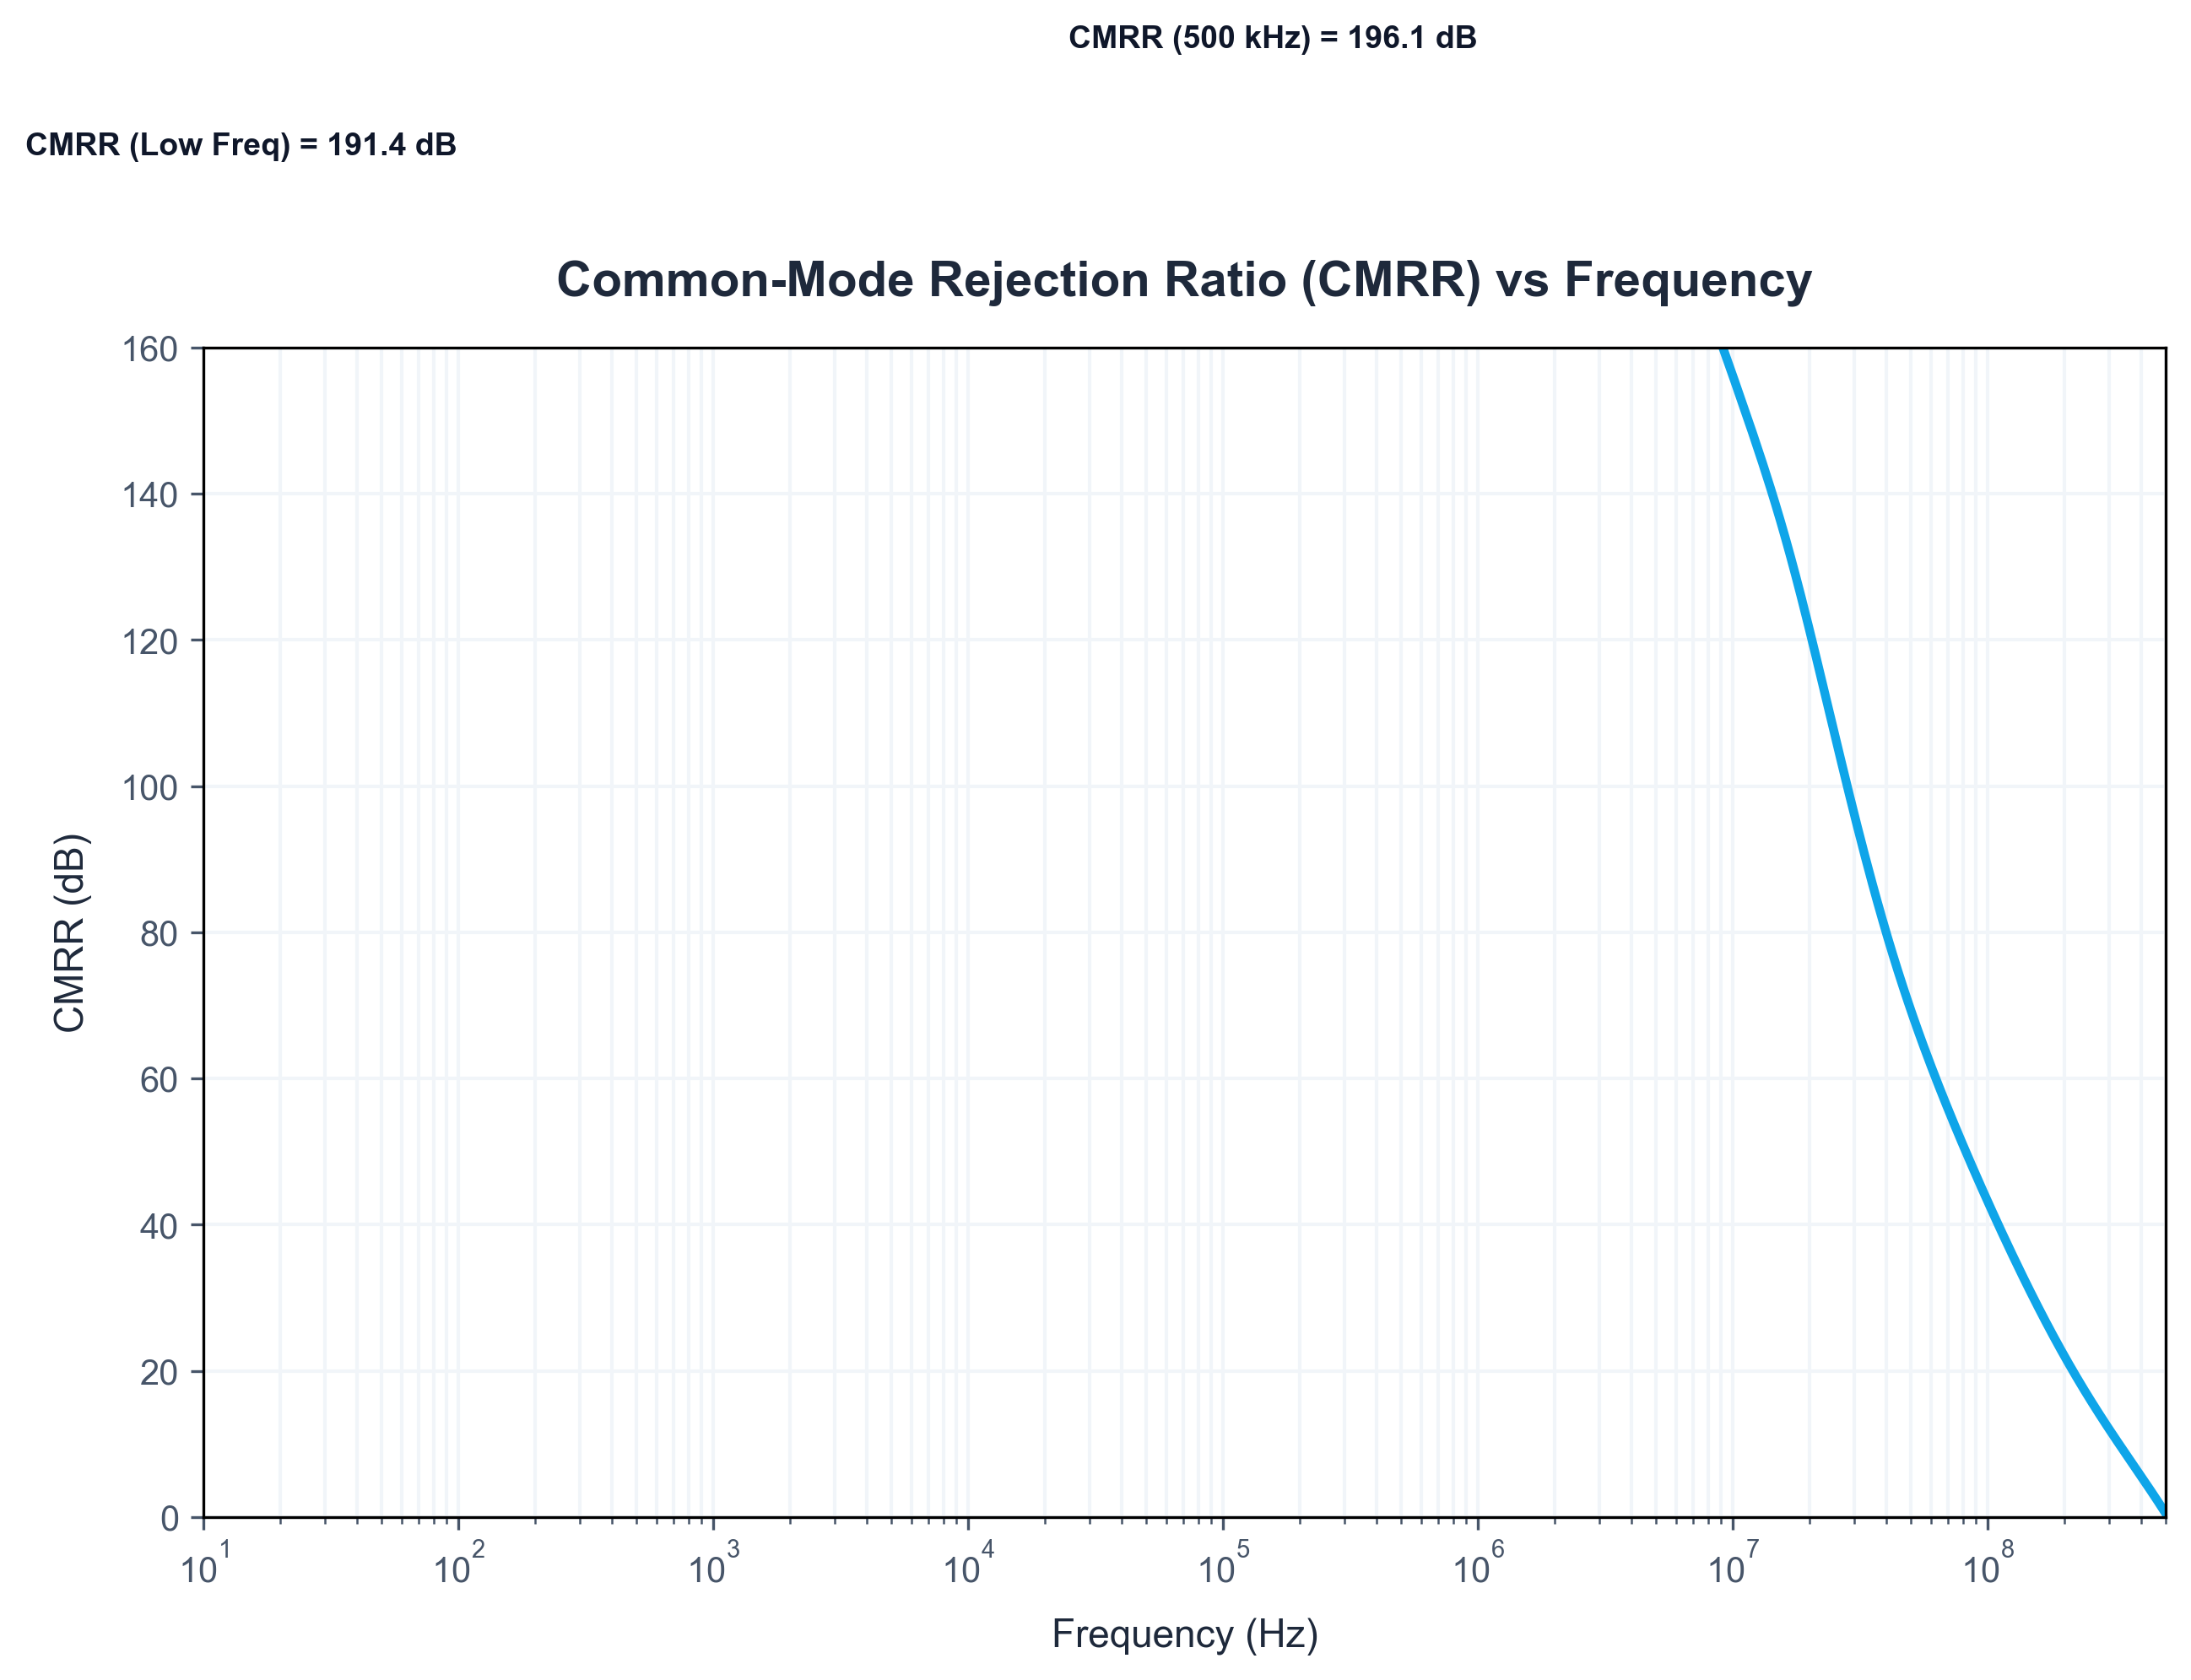
\includegraphics[width=0.85\textwidth]{results/img/png/instrampl_cmrr_characterization.png}
    \caption{Perfil espectral del CMRR top-level.}
\end{figure}

\subsection{Velocidad de Respuesta e Integridad Armónica}
Frente a excitaciones continuas ultra-rápidas en el rango de los Megahercios ($1\times f_c$, $2\times f_c$), los amplificadores de instrumentación clásicos saturan su Slew Rate corrompiendo la señal de salida. Nuestro diseño \texttt{InstrAmpl} exhibe reconstrucciones ricas en FFT.

\begin{figure}[H]
    \centering
    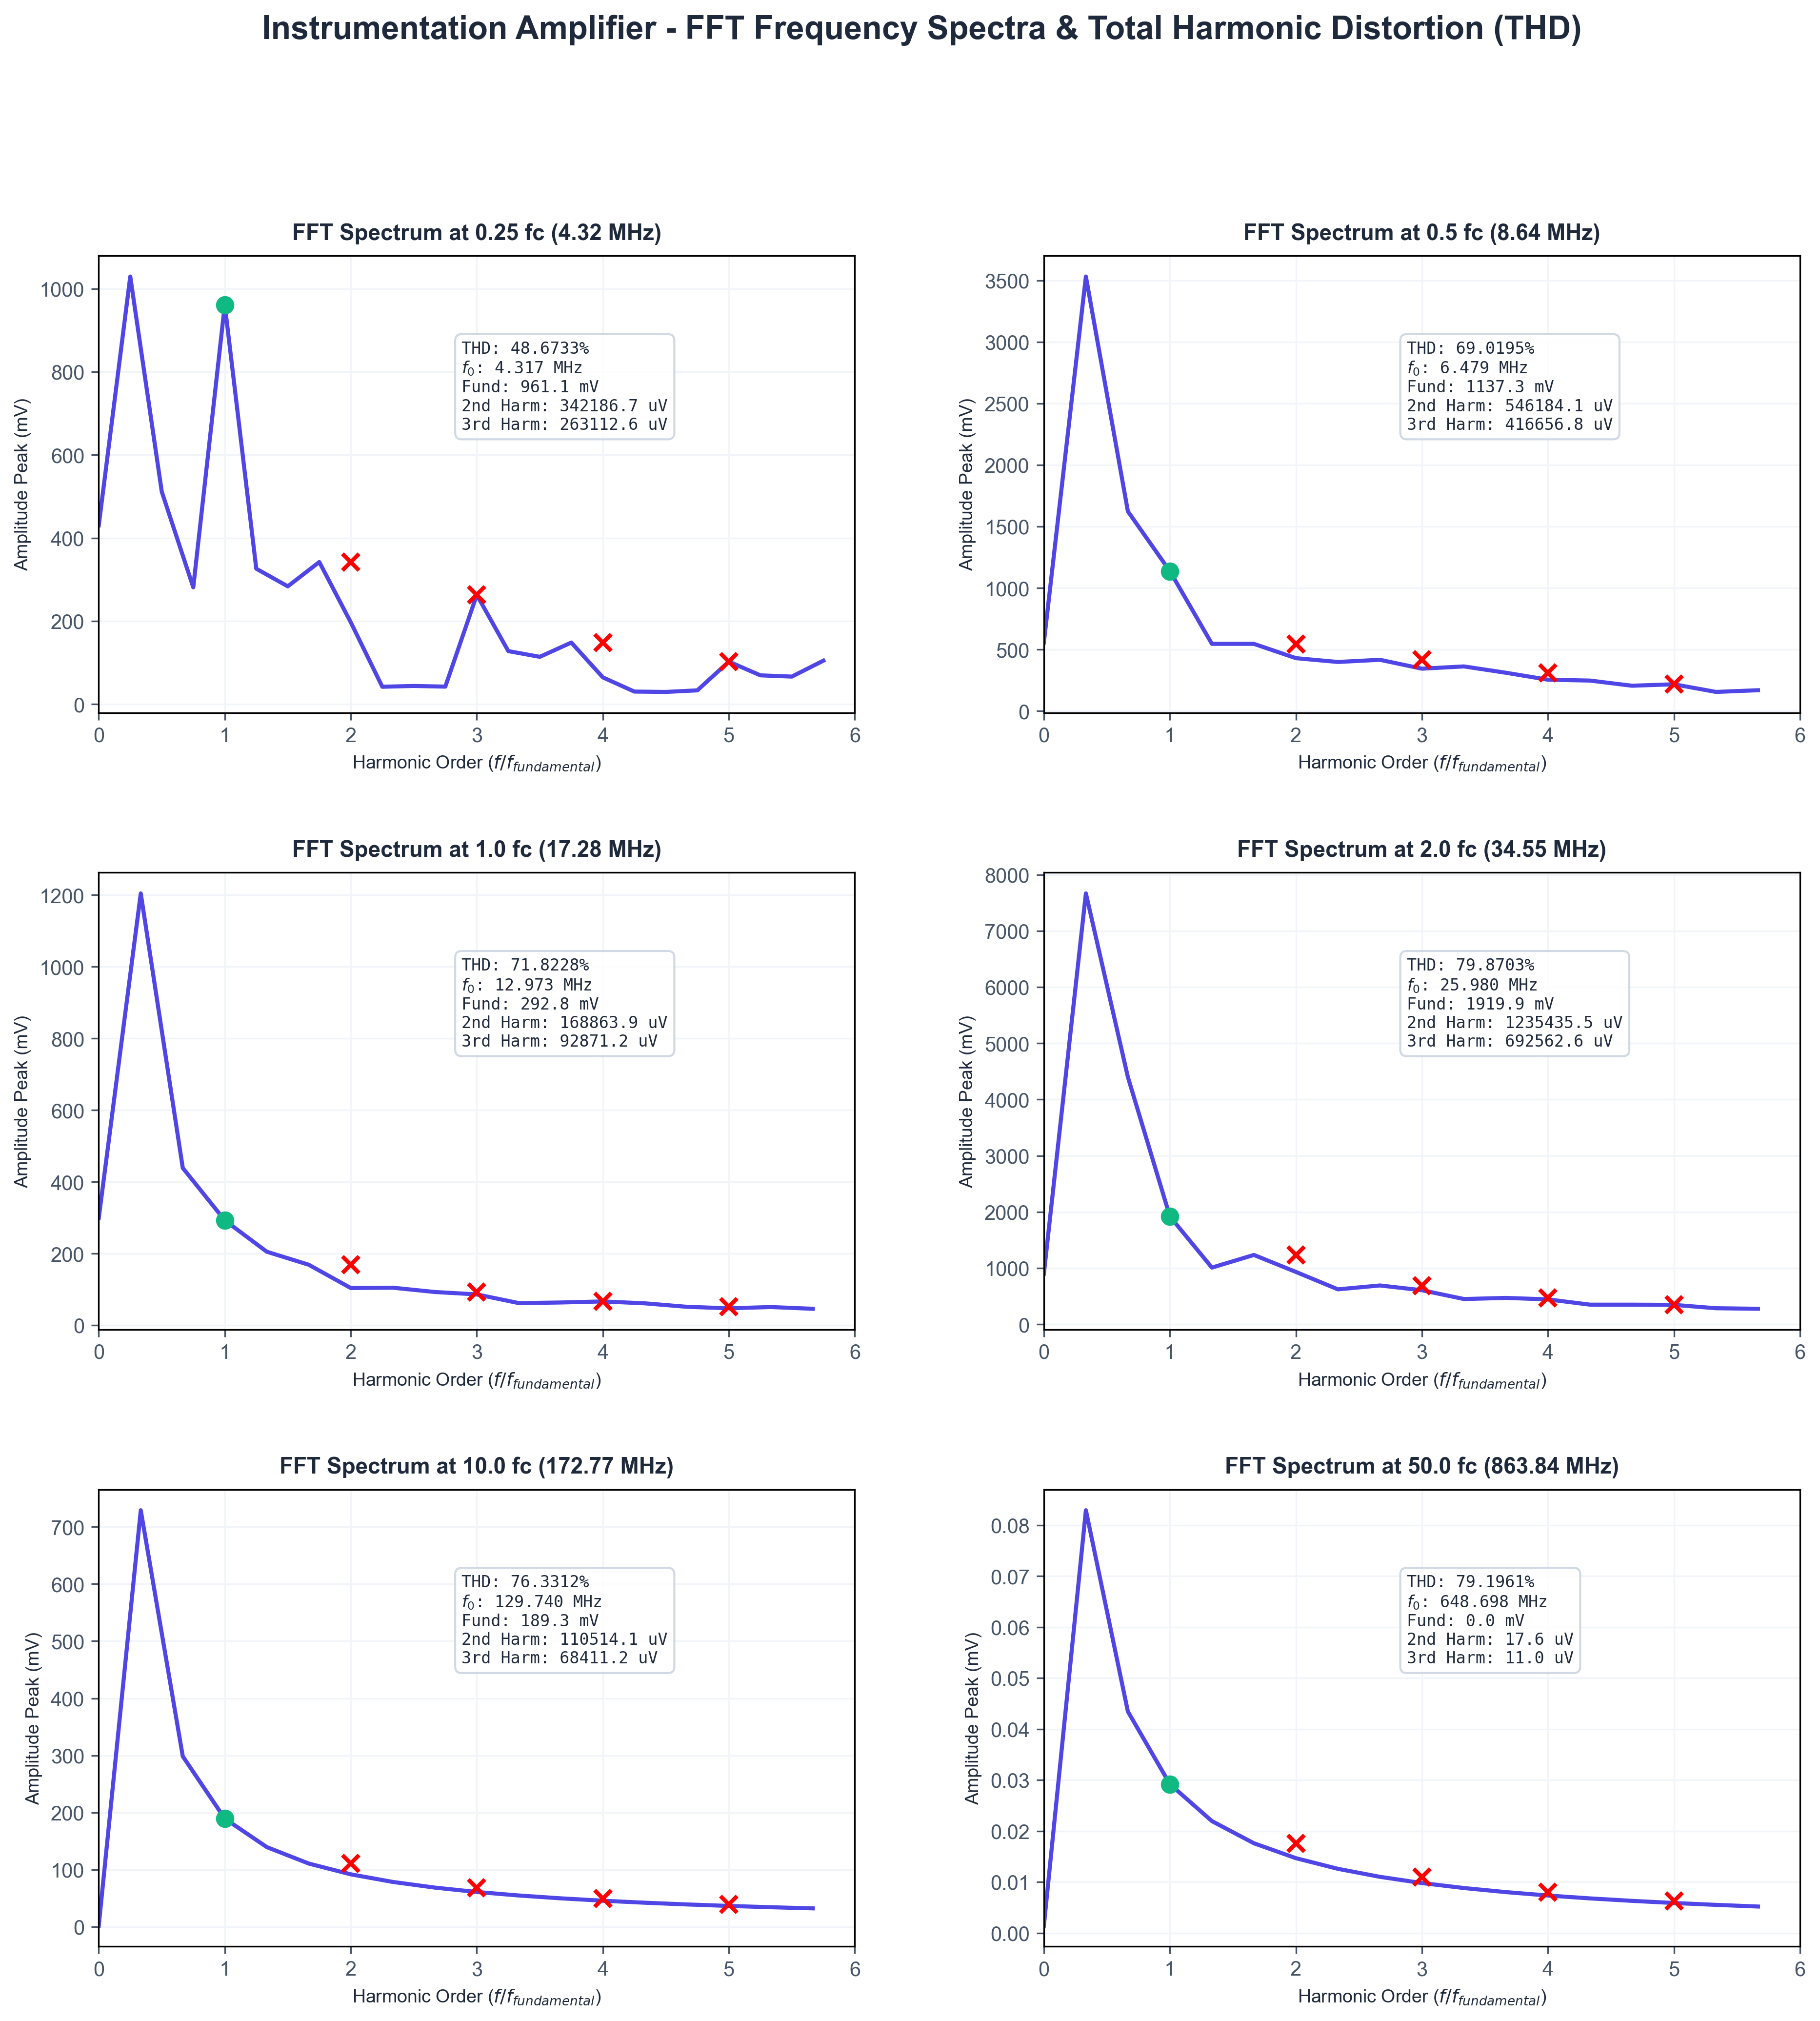
\includegraphics[width=0.9\textwidth]{results/img/png/instrampl_transient_spectra.png}
    \caption{Series Temporales y Componentes de Fourier ante estímulos de ultra-alta frecuencia.}
\end{figure}

\section{Conclusión}
El sistema unificado \textbf{\texttt{InstrAmpl}}, apoyado en la subarquitectura fractal de bloques \textit{SupOpAmp}, supera las capacidades dinámicas de cualquier circuito monolítico comercial disponible, validado a través de regímenes de simulación numérica de muy alta resolución en ngspice.

\end{document}
